\section{\sysname{}}
\label{sec:system}

\sysname{} addresses the application-specific adaptation by separating data
processing from degradation operations with \texttt{maybe} APIs. Developers
provide hints on potential operations that trade data fidelity with bandwidth
demand without being exact on the numbers. Instead, \sysname{} learns the
concrete degradation strategies using profiling data (either offline or online)
and controls the application execution adaptively. \autoref{fig:overview}
provides an overview of the systems and we will then describe each stage in
detail.

\begin{figure}
  \centering
  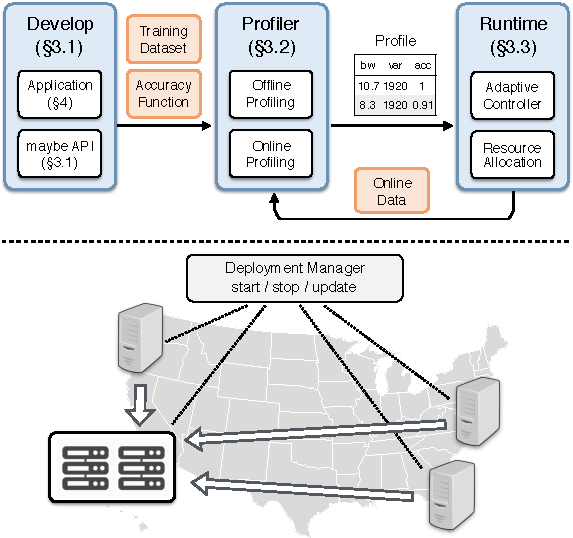
\includegraphics[width=.9\linewidth]{figures/system.pdf}
  \caption{\sysname{} Overview.}
  \label{fig:overview}
\end{figure}

\subsection{Structured Adaptation}
\label{sec:struct-adapt}

DAG: Applications are modelled as a directed acyclic graph (DAG) of
computation.  \texttt{maybe} operators to express the specification of
degradation. Our propose APIs do not require developers to be exact on the
quantity; integrating this into existing applications requires minimal effort.

We first consider a strawman solution: manual policies for
degradation. JetStream~\cite{rabkin2014aggregation} offers an example: ``if
bandwidth is insufficient, switch to sending images at 75\% fidelity, then 50\%
if there still isn't enough bandwidth. Beyond that point, reduce the frame rate,
but keep the images at 50\% fidelity.'' We identify the following issues with
this approach.

\para{Lack of precision:} These policies are often developer heuristics and
rarely backed up by measurements. First, there is no direct association of the
application accuracy with the 75\% fidelity configuration. Besides, their impact
on the data size is also not trivial.  While it seems intuitive that the level
of degradation will affect the data size, the precise impact is not always
straightforward. For example, one might think that reducing the frame rate by
50\% will half the data rate. When video encoding is employed, the inter-frame
difference will increased (P-frame size) when the frame rate is reduced. This
leads to a larger data size for each frame. \autoref{fig:h264} illustrates this
complex relationship with an example of H.264 encoding under four different
frame rates.

\para{Not scalable:} The strawman solution quickly leads to too many policies
when multiple degradation operations are involved or a fine-grained control is
desired. This manual process becomes tedious and error-prone. When too few rules
are provided, the application may oscillate between two rules: one that's too
aggressive (always faces insufficient bandwidth) and one that's too
conservative.

\para{Fixed:} Implemented as part of the application processing, it's fixed and
cannot be updated easily.

When using the above strawman solution, developers are forced to manually study
and measure the impact of individual degradation policy, prohibiting its wide
adoption in practice.

On the other extreme of the design spectrum, a completely developer-free
solution is not practical. While static analysis has been shown to optimize
application execution adaptively in a certain context~\cite{chun2011clonecloud},
they do not work well in our dataflow programming model. Static analysis is
prone to false positives: exploring wrong or unnecessary parameters. For
example, when the application is configured to generates statistics with a
\texttt{timed\_window} operation, static analysis may falsely detect the
duration parameter and alter the behavior of the application in an unexpected
way. Also, as we will illustrate in~\autoref{sec:profiling}, with each
introduced parameter, the profiling time increases drastically as all parameters
pose a combinatorial space.

Our system take a middle ground between these two extremes: developers use a
novel \texttt{maybe} API to annotate degradation operations without being exact
on the values. Think of these APIs as hints from developers: this operation,
when in use, will likely reduce the data size and affect the data fidelity;
however the exact impact is not clear.

The basic form of \texttt{maybe} operator takes two arguments: a knob and a
degradation function (see \autoref{tab:operators}). The knob indicates different
degradation levels; the function performs the actual degradation operation with
a configurable level. We restrict the type signature of the function that this
API can accept: $f(T, I) \Rightarrow I$. That is, the degradation function
should not alter the type of the stream. While this might seem a strong
restriction, when combined with \texttt{map} operator, the system is still
expressive enough. We describe our implementation and usage
in~\autoref{sec:implementation}.

Based on the \texttt{maybe} primitive, one can implement wrappers for common
degradation operations. For example, \texttt{maybe\_skip} will optionally
subsample a stream; and \texttt{maybe\_downsample} can adjust the image
resolution to a configured target. With this API, the example mentioned earlier
can now be implemented as follows:

\begin{lstlisting}
   let app = Camera::new((1920, 1080, 30))
      .maybe_downsample(vec![(1600, 900), (1280, 720)])
      .maybe_skip(vec![2, 5])
      .map(|frame| frame.show())
      .compose();
\end{lstlisting}

This snippet first instantiate a \texttt{Camera} source, which produces
\texttt{Stream<Image>} with 1920x1080 resolution and 30 FPS. Two degradation
operations are chained after the source: one that downsample the resolution to
either 1600x900 or 1280x720; the other skip the frame with a parameter of 2 or
5, resulting in 30/(2+1)=10 FPS or 30/(5+1)= 6 FPS. After the degradation,
images are shown on the display. In practice, further processing operators can
be chained.

While the API itself has simplified the specification of degradation, the exact
amount has to be known for precise rate adjustment at runtime. We then turn to
the second stage of our system that performs automatic profiling.

\begin{table*}
  \centering
  \begin{tabular}{ c r l }
    \toprule
    \multirow{7}{*}{Normal Operators}
    & \textit{map}(f: I $\Rightarrow$ O) & Stream<I> $\Rightarrow$ Stream<O> \\
    & \textit{filter}(f: I $\Rightarrow$ bool) & Stream<I> $\Rightarrow$
                                                 Stream<I> \\
    & \textit{skip}(i: Integer) & Stream<I> $\Rightarrow$ Stream<I> \\
    & \textit{sliding\_window}(count: Integer, f: Vec<I> $\Rightarrow$ O) & Stream<I> $\Rightarrow$
                                                                            Stream<O> \\
    & \textit{tumbling\_window}(count: Integer, f: Vec<I> $\Rightarrow$ O) & Stream<I> $\Rightarrow$
                                                                             Stream<O> \\
    & \textit{timed\_window}(time: Duration, f: Vec<I> $\Rightarrow$ O) & Stream<I> $\Rightarrow$
                                                                          Stream<O> \\
    & ... & ... \\
    \midrule
    \multirow{4}{*}{Degradation Operators}
    & \textit{maybe}(knobs: Vec<T>, f: (T, I) $\Rightarrow$ I) & Stream<I> $\Rightarrow$
                                                                 Stream<I> \\
    & \textit{maybe\_skip}(knobs: Vec<Integer>) & Stream<I> $\Rightarrow$ Stream<I> \\
    & \textit{maybe\_downsample}(knobs: Vec<(Integer, Interger)>) & Stream<Image> $\Rightarrow$ Stream<Image> \\
    & ... & ... \\
    \bottomrule
  \end{tabular}
  \caption{A comparison between normal stream processing operators and our
    degradation operators. \texttt{Vec<T>} represents a list of elements of type
    T. \texttt{Option<T>} indicates an optional element of type T which is
    either present \texttt{Some(T)} or absent \texttt{None}.}
  \label{tab:operators}
\end{table*}

\subsection{Automatic Profiling}
\label{sec:automatic-profiling}

The goal of our profiling stage is to explore the bandwidth-accuracy trade-off
and generate a \textit{profile} that is Pareto-optimal.

\subsubsection{Profiling Formalism}
\label{sec:formalize-profiling}

We first define terms and notations we will use. Each \texttt{maybe} operator
within an application corresponds to a knob $k$. Suppose the application has $n$
knobs, their combination forms a configuration $c = [k_{1}, k_{2},
... k_{n}]$. The set of all configurations $\mathbb{C}$ is the space that our
profiling system need to explore.

There are two mappings that we are particularly interested: a mapping from a
particular configuration to its bandwidth requirement $B(c)$ and the accuracy
measure $A(c)$. The Pareto-optimal set $\mathbb{P}$ can then be defined
(\autoref{eq:pareto}): for all $c \in \mathbb{P}$, there is no alternative
configuration $c'$ that requires less bandwidth while giving a higher accuracy.

{\small
\begin{equation}
  \mathbb{P} = \{ c \in \mathbb{C} : \{ c' \in \mathbb{C}: B(c') < B(c),
  A(c') > A(c) \} = \varnothing\}
  \label{eq:pareto}
\end{equation}
}%

\begin{table}
  \centering
  \begin{tabular}{r l}
    \toprule
    \textbf{Symbol} & \textbf{Description} \\
    \midrule
    $n$ & number of degradation operations \\
    $k_i$ & the \textit{i}-th degradation knob \\
    $c = [k_{1}, k_{2}, ... k_{n}]$ & one specific configuration \\
    $\mathbb{C}$ & the set of all configurations \\
    \midrule
    $B(c)$ & bandwidth requirement for $c$ \\
    $A(c)$ & accuracy measure for $c$ \\
    $\mathbb{P}$ & Pareto efficienct set \\
    \bottomrule
  \end{tabular}
  \caption{Notations used in profiling.}
  \label{tab:notations}
\end{table}

Since there is often no closed form relation for $B(c)$ and $A(c)$, our system
takes a data-driven approach: with a representative dataset and an
application-specific utility function, our system evaluates each configuration
for their bandwidth demand and accuracy degradation. The degradation could
either be measured against the groundtruth; or in the case when labelled dataset
is not available, the system uses the reference results when all degradations
are turned off.

\subsubsection{Offline Profiling}
\label{sec:offline-profiling}

Users provide a representative training data set. \para{Profiling is costly, ok
  for offline.}

\subsubsection{Online Profiling}
\label{sec:online-profiling}

When doing online profiling, we face two challenges: 1, lack of original data;
2, efficient profiling.

\para{Lack of groundtruth data or reference data.} During the online execution,
it's often not feasible to get groundtruth labelled data. Even with the
undegraded data may not be available.

\begin{itemize}[leftmargin=16pt]
\item Allocate some bandwidth for portions of undegraded data.
\item Use current best data as reference.
\end{itemize}

Although the first scheme seems to be incurring unnecessary bandwidth
consumption, when the runtime is probing for bandwidth, the data can enjoy a
free ride.

\para{Efficient profiling.} When doing profiling online, exhaustive exploring
all configurations is costly.

\begin{itemize}[leftmargin=16pt]
\item Parallel execution.
\item Smaller chunk of data.
\item Triggering profiling.
\end{itemize}

\subsection{Runtime Adaptation}
\label{sec:runtime}

At runtime, \sysname{} performs application adaptation according to the learned
profile. We choose to design our own runtime system and adaptation algorithm
because prior solutions are not satisfactory: $(i)$~network protocols adapt to
available resources without application accuracy guarantee; $(ii)$
JetStream~\cite{rabkin2014aggregation} uses manual policies and doesn't support
degradations along multiple dimensions; and $(iii)$~video streaming adaptation,
such as Huang et al.~\cite{huang2014buffer}, uses the playback buffer and incurs
high latency.

Our runtime differs from prior systems in the ability to react
with precision: it stays in a low-latency state and uses a Pareto-optimal
configuration for high accuracy.

\begin{figure}
  \centering
  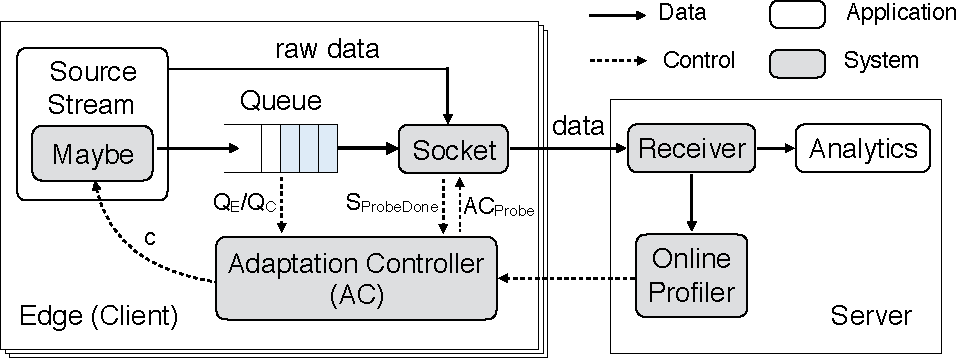
\includegraphics[width=\linewidth]{figures/runtime-adaptation.pdf}
  \caption{Runtime adaptation system architecture.}
  \label{fig:runtime}
\end{figure}

\autoref{fig:runtime} shows our runtime system architecture. \sysname{}
applications' source contains a \texttt{Maybe} module derived from all \maybe{}
operations. This module allows the controller to update the level of
degradation. Data generated by the source is then enqueued to \texttt{Queue} and
subsequently dequeued by \texttt{Socket}. When the data generation rate exceeds
\texttt{Socket}'s departure rate, the queue grows. In this case, the adaptation
controller (AC) queries the estimated bandwidth from \texttt{Socket} and
regulates the source stream by updating the configuration.  After the data is
sent through the network, the receiver extracts raw data to the online profiler
and delivers data to the application analytics. Raw data is only transmitted
when the queue is empty. When a new profile is learned, it is fed back to AC for
subsequent adaptation.

We then describe the adaptation algorithm; \autoref{fig:cc} shows the state
machine model and an example trace for illustration.  AC loads the profile and
sorts all configurations with an ascending order of bandwidth demand, resulting
in a list $[c_1, \dots, c_{\max}]$.  These configurations follow a total order:
$c_i < c_j$ if $B(c_i) < B(c_j)$.  We denote the current configuration as $c_i$
and the next $c_{i+1}$.  AC receives messages from the \texttt{Queue}: message
\qe{} when the queue is empty and $\text{Q}_\text{C}$ when queued items exceed a
threshold. AC can query \texttt{Socket} for delivery rate $R$ or request it to
probe ($\text{AC}_{\text{Probe}}$) for a target bandwidth, often
$B(c_{i+1})$. When $R > B(c_{i+1})$, \texttt{Socket} sends back \spd{}. The
algorithm follows a state machine as described below:

\begin{itemize}[leftmargin=*, topsep=3pt, itemsep=0pt]

\item \textbf{Startup: rapid growth.} \sysname{} starts with $c_1$ and grows the
  rate ($c_i \Rightarrow c_{i+1}$) upon each \qe{}. The growth stops at
  $c_{\max}$ (to \texttt{Steady}) or if it receives \qc{} (to \texttt{Degrade}).

\item \textbf{Degrade: reacting to congestion.} When \texttt{Queue} grows and
  exceeds a threshold, AC receives \qc{} and runs the \texttt{adapt()}
  procedure. This involves two steps: (1) AC queries $R$ from \texttt{Socket};
  (2) AC updates \texttt{Maybe} with the maximum-allowed $c$ that satisfies
  $B(c) < \alpha R, \alpha \in (0, 1)$. A smaller $\alpha$ allows a quicker
  draining of the queue. After the queue is drained, \sysname{} changes to
  \texttt{Steady}.

\item \textbf{Steady: low latency delivery.} \sysname{} achieves low latency by
  spending most of the time in the \texttt{Steady} state. It changes to
  \texttt{Degrade} when congestion occurs. If $c < c_{\max}$ and it receives
  \qe{}, AC enters the \texttt{Probe} state to check for more available
  bandwidth.

\item \textbf{Probe: more bandwidth for a higher accuracy.} Advancing the configuration
  directly causes a drastic latency increase when $B(c_{i+1}) \gg B(c_i)$. To
  allow a smooth increase, AC requests \texttt{Socket} to probe by sending
  additional traffic controlled by \texttt{probe\_gain} (in
  \texttt{inc\_pace()}, similar to BBR~\cite{cardwell2017bbr}). \sysname{} stops
  probing under two conditions: (1) upon \spd{}, it advances $c_i$; (2) upon
  \qc{}, it returns to \texttt{Steady}.

\end{itemize}

\begin{figure}
  \begin{subfigure}[t]{\columnwidth}
    \centering
    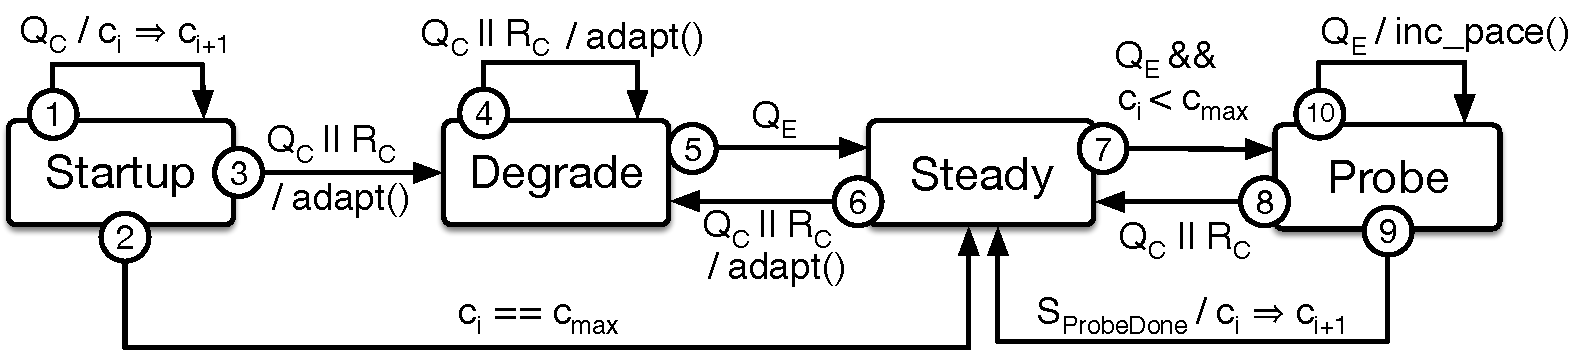
\includegraphics[width=\columnwidth]{figures/cc.pdf}
    \caption{Rate adaptation as a state machine.}
    \vspace{1em}
    \label{fig:cc-sm}
  \end{subfigure}
  \begin{subfigure}[t]{\columnwidth}
    \centering
    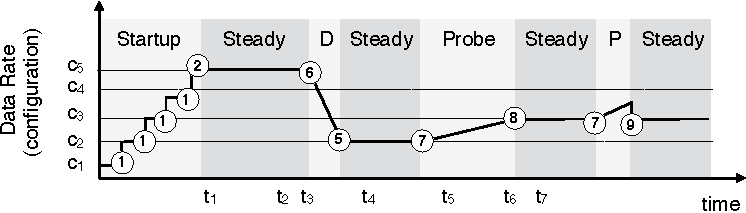
\includegraphics[width=\columnwidth]{figures/cc2.pdf}
    \caption{An example illustrating the adaptation algorithm.}
    \label{fig:cc-ex}
  \end{subfigure}
  \caption{Runtime adaptation algorithm.}
  \label{fig:cc}
\end{figure}

% \begin{figure}
%   \centering
%   \resizebox{\columnwidth}{!}{
%     \begin{tikzpicture}[
  state/.style = { draw, very thick, fill=white, rounded corners=1em,
    minimum height=3em, minimum width=7em, node distance=7em, font={\bfseries},
    align=center },
  edge portion/.style = { black, thick },
  transition/.style = { edge portion, -> },
  algorithm/.style = { draw, thin, fill=white },
  ]

  \node [state] (startup) {
    STARTUP };
  \node [state] (congestion) [right=of startup] {CONGESTION};
  \draw [transition] (startup) -- (congestion)
  node [midway, auto] {Q.Congestion};

  \node [state] (steady) [below=of congestion] {STEADY};

  \draw [transition] ($(congestion.south west)!0.4!(congestion.south east)$)
  to node[midway, sloped, below] {Q.NoQueue}
  ($(steady.north west)!0.4!(steady.north east)$);

  \draw [transition] ($(steady.north west)!0.6!(steady.north east)$)
  to node[midway, sloped, below] {Q.Congestion}
  ($(congestion.south west)!0.6!(congestion.south east)$);

  \node [state] (probe) [left=of steady] {PROBE};

  \draw [transition] ($(steady.south west)!0.6!(steady.north west)$)
  -- ($(probe.south east)!0.6!(probe.north east)$)
  node[midway, auto, swap] {Q.Probe};

  \draw [transition, <-] ($(steady.south west)!0.4!(steady.north west)$)
  -- ($(probe.south east)!0.4!(probe.north east)$)
  node[midway, auto, align=left] {Q.Congestion | \\ IO.ProbeDone};

\end{tikzpicture}


%%% Local Variables:
%%% mode: latex
%%% TeX-master: "sosp17"
%%% End:

%   }
%   \caption{Congestion Control Algorithm}
%   \label{fig:cc}
% \end{figure}

\para{Resource Allocation and Fairness.} In addition to rate adaptation, the
profile is also useful for controlling a single application's bandwidth usage or
allocating resources among competing tasks.

For individual applications, developers can pinpoint a configuration for a given
bandwidth or accuracy goal. They can also specify a criterion to limit effective
configurations. For example, \sysname{} can enforce an upper bound on the
bandwidth consumption, useful to reduce WAN bandwidth usage and cost.

For multiple applications, their profiles allows novel bandwidth allocation
schemes such as utility fairness. Different from traditional resource fairness
where applications get equal share of bandwidth, utility fairness aims
to maximize the \textit{minimal} application accuracy. With the profiles,
finding allocations is equivalent to finding proper configuration $c^t$ for
application $t$. We formulate utility fairness as follows:

%% Pick one based on the space

\begin{equation}
 \label{eq:multitask}
 \underset{c^t}{\max} \; \min({A^t(c^t)})
 \;
 \text{s.t.}
 \;
 \sum_t{B^t(c^t)} < R
\end{equation}

% \begin{equation}
%  \label{eq:multitask}
%  \begin{aligned}
%     & \underset{c^t}{\text{maximize}} & & \min({A^t(c^t)}) & & \\
%     & \text{subject to} & & \sum_t{B^t(c^t)} < R & & \\
%  \end{aligned}
% \end{equation}

Solving this optimization is computationally hard. \sysname{} uses a heuristics
approach. We start with $c_1^t$ and improve the application $t$ that has the
worst accuracy. This process repeats until we have allocated all available
bandwidth.

%%% Local Variables:
%%% mode: latex
%%% TeX-master: "awstream"
%%% End:


%%% Local Variables:
%%% mode: latex
%%% TeX-master: "sosp17"
%%% End:
